\documentclass[reqno]{amsart}

\usepackage{amsfonts,latexsym,amsthm,amssymb,amsmath,amscd,euscript,bm}
\usepackage[sc]{mathpazo}
\usepackage[margin = 2.6cm]{geometry}
\usepackage{enumitem}
\usepackage{hyperref}
% sets numbering of enumerate to a, b, c, ...
\renewcommand{\theenumi}{\alph{enumi}}

% Theorems, propositions, etc.
\newtheorem{theorem}{Theorem}
\newtheorem{proposition}[theorem]{Proposition}
\newtheorem{lemma}[theorem]{Lemma}
\newtheorem{corollary}[theorem]{Corollary}

\theoremstyle{definition}
\newtheorem{definition}[theorem]{Definition}
\newtheorem*{claim}{Claim}

\theoremstyle{remark}
\newtheorem*{remark}{Remark}
\newtheorem*{notation}{Notation}

\usepackage{tikz-cd}

\usepackage{graphicx}

% Math blackboard font
\newcommand{\nc}{\newcommand}
\nc{\on}[1]{\operatorname{#1}}

\nc{\R}{\mathbb R}
\nc{\C}{\mathbb C}
\nc{\Q}{\mathbb Q}
\nc{\Z}{\mathbb Z}
\nc{\N}{\mathbb N}
\nc{\HH}{\mathbb H}
\nc{\DD}{\mathbb D}
\nc{\TT}{\mathbb T}
\nc{\EE}{\mathbb E}
\nc{\PP}{\mathbb P}

\nc{\cT}{\mathcal T}
\nc{\cA}{\mathcal A}
\nc{\cM}{\mathcal M}
\nc{\cR}{\mathcal R}
\nc{\cB}{\mathcal B}
\nc{\cG}{\mathcal G}
\nc{\cD}{\mathcal D}
\nc{\cS}{\mathcal S}
\nc{\cF}{\mathcal F}
\nc{\cL}{\mathcal L}
\nc{\cE}{\mathcal E}

\nc{\diam}{\operatorname{diam}}
\nc{\supp}{\operatorname{supp}}
\nc{\loc}{\text{loc}}
\nc{\pv}{\operatorname{pv}}

% Why the f*** would you ever use \epsilon
\renewcommand{\epsilon}{\varepsilon}
\renewcommand{\emph}{\textsc}

\renewcommand{\Re}{\operatorname{Re}}
\renewcommand{\Im}{\operatorname{Im}}
%inverse Fourier transform widecheck
\DeclareFontFamily{U}{mathx}{\hyphenchar\font45}
\DeclareFontShape{U}{mathx}{m}{n}{
      <5> <6> <7> <8> <9> <10>
      <10.95> <12> <14.4> <17.28> <20.74> <24.88>
      mathx10
      }{}
\DeclareSymbolFont{mathx}{U}{mathx}{m}{n}
\DeclareFontSubstitution{U}{mathx}{m}{n}
\DeclareMathAccent{\widecheck}{0}{mathx}{"71}

\let\vec\mathbf

% Title: change problem set number as needed
\title
{
	\emph{Integral operators}
} 

\author{Jason Zhao}
\date{\today}

\begin{document}
\maketitle

\begin{abstract}
	This article surveys the study of linear operators taking the form 
		\[ Tf(y) := \int_{\R^d} K(x, y) f(x) \, dx \]
	where $K : \R^d \times \R^d \to \C$ is known as the \textit{kernel} of the \textit{integral operator} $T$. A fundamental problem in harmonic analysis is determining the boundedness of the operator $T$ between function spaces given certain conditions on the kernel $K$. This has applications in establishing the Sobolev embedding inequalities and energy estimates for linear PDE. Standard references include \cite{Duoandikoetxea2001} and \cite{Stein1970}. 
\end{abstract}

\tableofcontents

\section{Schur's test}

Let $(X, \mu)$ and $(Y, \nu)$ be measure spaces, and let $K : X \times Y \to \C$ be a measurable function. Formally, an \emph{integral operator} is a linear operator of the form
	\[ Tf(y) := \int_X K(x, y) f(x) \, d\mu (x) \]
mapping a function $f: X \to \C$ to a function $Tf : Y \to \C$. The function $K$ is known as the \emph{kernel} of the integral operator $T$. A priori, the integral on the right is not well-defined, motivating the introduction various integrability conditions on $K$, which upon appealing to Minkowski's integral inequality or Holder's inequality we see that the integral defining $Tf(y)$ converges absolutely for almost every $y \in Y$. Furthermore, we can show that $T$ forms a bounded operator between Lebesgue spaces.

\subsection{Strong-type integrability conditions}

Assuming uniform $L^1$-integrability conditions on $K(x, y)$ in $x$ and $y$, we can show that $T$ satisfies a strong-type $(1, 1)$ and $(\infty, \infty)$ inequality, which by complex interpolation \textit{a la} Riesz-Thorin would furnish a strong-type $(p, p)$ inequality. This is the classical statement of Schur's test, which is the particular case on the diagonal of the general Schur's test stated below:

\begin{theorem}[Strong-type Schur's test]
	Suppose that $K: X \times Y \to \C$ obeys the bounds
		\begin{align*}
			 ||K (x, y) ||_{L^{q_0}_y (Y)} &\leq B_0 \qquad \text{uniformly for a.e. $x \in X$},\\
			 ||K(x, y)||_{L^{p_1'}_x (X)} &\leq B_1 \qquad \text{uniformly for a.e. $y \in Y$},
		\end{align*}	 
	for some constants $B_0, B_1 > 0$ and exponents $1 \leq p_1, q_0 \leq \infty$. Setting $p_0 := 1$ and $q_1 := \infty$, define the exponents $1 \leq p_\theta, q_\theta \leq \infty$ for $0 < \theta < 1$ by 
		\[ \frac{1}{p_\theta} = \frac{1 - \theta}{p_0} + \frac{\theta}{p_1}, \qquad \frac{1}{q_\theta} = \frac{1 - \theta}{q_0} + \frac{\theta}{q_1}. \]
	Then the integral operator $T$ satisfies the strong-type $(p_\theta, q_\theta)$ inequality
		\[ ||Tf||_{L^{q_\theta} (Y)} \leq B_0^\theta B_1^{1 - \theta} ||f||_{L^{p_\theta} (X)}. \]
\end{theorem}

\begin{proof}
	We argue by complex interpolation. The strong-type $(1, q_0)$ inequality follows from the triangle inequality and Minkowski's integral inequality, 
		\[ ||T f||_{L^{q_0} (Y)} \leq \left|\left| \int_X |K(x, y)| \, |f(x)| \, d\mu(x)  d \nu(y) \right|\right|_{L^{q_0}_y (Y)} \leq \int_X ||K (x, y) ||_{L^{q_0}_y (Y)} |f(x)| \, d \mu(x) \leq B_0 ||f||_{L^1 (X)} . \]
	The strong-type $(p_1, \infty)$ inequality follows from Holder's inequality
		\[ ||Tf||_{L^{\infty} (Y)} \leq \sup_{y \in Y} ||K(x, y)||_{L^{p_1'}_x (X)} ||f||_{L^{p_1} (X)} \leq B_1 ||f||_{L^{p_1} (X)}.\]	
	We conclude the desired strong-type $(p_\theta, q_\theta)$ inequality for $0 < \theta < 1$ via Riesz-Thorin interpolation. 
\end{proof}

\begin{remark}
	Note that we did not exploit the sign of the kernel $K$ anywhere in the proof of Schur's test, which suggests that Schur's test is ill-equipped for dealing with kernels exhibiting oscillation, such as the Fourier transform which has kernel $K(x, y) := e^{2\pi i x \cdot y}$, or cancellation, such as the Riesz transform which has kernel $K(x, y) := \tfrac{x_i - y_i}{|x - y|^{d + 1}}$. 
\end{remark}

\begin{corollary}[Strong-type Schur's test, diagonal]
	Suppose that $K: X \times Y \to \C$ obeys the bounds
		\begin{align*}
			 \int_X |K(x, y)| d \mu(x) &\leq A \qquad \text{uniformly for a.e. $y \in Y$},\\
			  \int_Y |K(x, y)| d \nu(y) &\leq B \qquad \text{uniformly for a.e. $x \in X$},
		\end{align*}	 
	for some constants $A, B > 0$. Then for $1 \leq p \leq \infty$ the integral operator $T$ satisfies the strong-type $(p, p)$ inequality 
		\[ ||Tf||_{L^p (Y)} \leq A^{1/p'} B^{1/p} ||f||_{L^p (X)}. \]
\end{corollary}

\begin{corollary}[Young's convolution inequality]
	Let $1 \leq p, q, r \leq \infty$ satisfy
		\[ \frac1p + \frac1q = \frac1r + 1. \]
	Then 
		\[ ||f * g||_{L^r (\R^d)} \leq ||f||_{L^p (\R^d)} ||g||_{L^q (\R^d)}. \]	
\end{corollary}

\begin{proof}
	The result follows from the strong-type Schur's test for kernel $K(x, y) := g(x - y)$ where $g \in L^q (\R^d)$. Since the $L^q$-norm is translation invariant, we have
		\[ ||K(x, y)||_{L^q_x} =  ||K(x, y)||_{L^q_y} = ||g||_{L^q}.  \]
	Working through the exponent numerology, we conclude Young's convolution inequality. 	
\end{proof}

\subsection{Weak-type integrability conditions}

If we replace the strong Lebesgue integrability conditions in the strong-type Schur's test by weak Lebesgue integrability conditions, we can use real interpolation to formulate a weak-type analogue of Schur's test:

\begin{theorem}[Weak-type Schur's test]
	Suppose that $K : X \times Y \to \C$ obeys the bounds
		\begin{align*}
			|| K(x, y) ||_{L^{q_0, \infty} (Y)} &\leq B_0 \qquad \text{uniformly for a.e. $x \in X$},\\
			 || K(x, y) ||_{L^{p_1', \infty} (X)} &\leq B_1 \qquad \text{uniformly for a.e. $y \in Y$},
		\end{align*}	
	for some constants $B_0, B_1 > 0$ and exponents $1 < p_1, q_0 < \infty$. Setting $p_0 := 1$ and $q_1 := \infty$, define the exponents $1 < p_\theta, q_\theta < \infty$ for $0 < \theta < 1$ by 
		\[ \frac{1}{p_\theta} = \frac{1 - \theta}{p_0} + \frac{\theta}{p_1}, \qquad \frac{1}{q_\theta} = \frac{1 - \theta}{q_0} + \frac{\theta}{q_1}. \]
	Then the integral operator $T$ satisfies the strong-type $(p_\theta, q_\theta)$ inequality
		\[ ||Tf||_{L^{q_\theta} (Y)} \lesssim_{p_1, q_0, \theta} B_0^\theta B_1^{1 - \theta} ||f||_{L^{p_\theta} (X)}. \] 
\end{theorem}

\begin{proof}
	We argue by real interpolation. The restricted weak-type $(1, q_0)$ and $(p_1, \infty)$ inequalities follow from the triangle inequality and Fubini-Tonelli, 
		\begin{align*}
			 \int_Y |T\mathbb 1_E (y)| \, \mathbb 1_F (y) \, d \nu(y) 
			 	\leq \int_F \left(\int_E |K(x, y)| \, d\mu(x) \right) d \nu(y) \leq B_1 \mu(E)^{1/p_1} \nu(F), \\
			  \int_Y |T\mathbb 1_E (y)| \, \mathbb 1_F (y) \, d \nu(y) 
			 	\leq  \int_E \left(\int_F |K(x, y)| \, d \nu(y) \right) d\mu(x)  \leq B_0 \nu(F)^{1/q_0'} \mu(E),
		\end{align*}	 
	for all measurable $E \subseteq X$ and $F \subseteq Y$. We conclude the desired strong-type $(p_\theta, q_\theta)$ inequality for $0 < \theta < 1$ via Marcinkiewicz interpolation. 	
\end{proof}

\begin{remark}
	Note that we needed to exclude the endpoints $p_1, q_0 = 1, \infty$ to use real interpolation. In particular, the weak-type Schur's test cannot furnish strong-type bounds on the diagonal. 
\end{remark}

\begin{corollary}[Weak-type Young's convolution inequality]
	Let $1 < p, q, r < \infty$ satisfy
		\[ \frac1p + \frac1q = \frac1r + 1. \]
	Then 
		\[ ||f * g||_{L^r (\R^d)} \lesssim_{p, q} ||f||_{L^p (\R^d)} ||g||_{L^{q, \infty} (\R^d)} \]	
	uniformly in $f \in L^p (\R^d)$ and $g \in L^{q, \infty} (\R^d)$.
\end{corollary}

\begin{proof}
	The result follows from the weak-type Schur's test for kernel $K(x, y) := g(x - y)$ where $g \in L^{q, \infty} (\R^d)$. Since the $L^{q, \infty}$-norm is translation invariant, we have 
		\[ ||K(x, y)||_{L^{q, \infty}_x} = ||K(x, y)||_{L^{q, \infty}_y} = ||g||_{L^{q, \infty}}. \]
	Working through the numerology, we conclude the weak-type Young's convolution inequality.	
\end{proof}

A useful application of the weak-type Schur's test to partial differential equations is in proving the Hardy-Littlewood-Sobolev inequality. Let $X = Y = \R^d$ and define
	\[ g(x) := \frac{1}{|x|^\alpha} \]
for $0 < \alpha < d$. Observe that $g \not\in L^p (\R^d)$ for any $1 \leq p \leq \infty$, so we cannot apply the strong-type Schur's test. On the other hand, $g \in L^{d/\alpha, \infty} (\R^d)$, so it follows from the weak-type Young's convolution inequality that

\begin{corollary}[Hardy-Littlewood-Sobolev]
	Let $1 < p < r < \infty$ and $0 < \alpha < d$ satisfy 
		\[ \frac1p + \frac{\alpha}{d} = 1 + \frac1r.\]
	Then 
		\[ || f * |x|^{-\alpha} ||_{L^r} \lesssim ||f||_{L^p} \]
	uniformly in $f \in L^p (\R^d)$. 		
\end{corollary}

\section{Calderon-Zygmund theory}

We turn our attention to kernels $K : \R^d \times \R^d \to \C$ which are \textit{singular} along the diagonal $x = y$. More precisely, we are interested in kernels which ``barely'' fail to be integrable, the prototypical example of which is the kernel
	\[ K(x, y) := \frac1\pi \frac{1}{y - x}. \]
Integrating in either $x$ or $y$, we see that $K$ admits a logarithmic singularity in the regions near the diagonal $|x - y| \ll 1$ and away from the diagonal $|x - y| \gg 1$. It is therefore not clear whether the integral operator corresponding to $K$, known as the \emph{Hilbert transform},
	\[ H f(y) := \frac1\pi \int_\R \frac{f(x)}{y - x} \, dx \]
is well-defined. Nonetheless, we can view $H$ as an integral operator ``away from the diagonal'', observing that the integral converges absolutely when $f \in L^2 (\R)$ is compactly supported and $x$ lies outside of the support of $f$. 

\subsection{Calderon-Zygmund operators}

A \emph{Calderon-Zygmund kernel} is a function $K : \R^d \times \R^d \to \C$ satisfying the \emph{Hormander condition}:
	\begin{align*}
		\int_{|x - y| > 2|y - z|} |K(x, y) - K(x, z)| \, dx &\lesssim 1 \qquad \text{uniformly for a.e. $y \neq z$}, \\
		\int_{|x - y| > 2|x - w|} |K(x, y) - K(w, y)| \, dy &\lesssim 1 \qquad \text{uniformly for a.e. $x \neq w$}.
	\end{align*}
We say that a bounded linear operator $T: L^2 (\R^d) \to L^2 (\R^d)$ is a \emph{Calderon-Zygmund operator} if there exists a Calderon-Zygmund kernel $K$ for which 
	\begin{equation}
		Tf(y) = \int_{\R^d} K(x, y) f(x) \, dx \tag{*} \label{eq:intCZO}
	\end{equation}
whenever $f \in L^2 (\R^d)$ is compactly supported and $y$ lies outside the support of $f$. 

\begin{remark}
The Hormander condition is sometimes known as a \textit{smoothness} condition, as it is often stated in the form of the strictly stronger Holder-type regularity assumptions
	\begin{align*}
			|K(x, y) - K(x, z)| 
				&\lesssim \frac{|y - z|^\delta}{|x - y|^{d + \delta}},	\qquad \text{whenever } |x - y| > 2|y - z|,\\
			|K(x, y) - K(w, y)| 
				&\lesssim \frac{|x - w|^\delta}{|x - y|^{d + \delta}},	\qquad \text{whenever } |x - y| > 2|x - w|	,
		\end{align*}
for some Holder exponent $0 < \delta \leq 1$. When $\delta = 1$, these form Lipschitz-type regularity estimates, which in turn are implied via the fundamental theorem of calculus by the gradient estimates
	\begin{align*}
		|\nabla_x K(x, y)| 
			&\lesssim \frac{1}{|x - y|^{d + 1}}, \\
		|\nabla_y K(x, y)|
			&\lesssim \frac{1}{|x - y|^{d + 1}}.	
	\end{align*}
\end{remark}

	The integral representation (\ref{eq:intCZO}) does not fully characterise a Calderon-Zygmund operator. For example, the derivative operator $Tf(y) := f'(y)$ has kernel zero, however it is not a bounded operator on $L^2 (\R)$. Furthermore, for any $b \in L^\infty (\R^d)$ the multiplication operator $Tf(y) := b(y) f(y)$ is a Calderon-Zygmund operator with kernel zero. Fortunately, this is the only source of ambiguity:

\begin{proposition}
	If $T_1, T_2 : L^2(\R^d) \to L^2 (\R^d)$ are Calderon-Zygmund operators associated to the same kernel, then they differ by a pointwise multiplication operator $(T_1 - T_2) f = b f$ for some $b \in L^\infty (\R^d)$. 
\end{proposition}

\begin{proof}
	By linearity it suffices to show that a Calderon-Zygmund operator $T: L^2 (\R^n) \to L^2 (\R^d)$ corresponding to the zero kernel takes the form $Tf(y) = b(y) f(y)$ for some $b \in L^\infty (\R^d)$. Observe that the measure 
		\[ E \mapsto \int_E T \mathbb 1_E (y) \, dy \]
	is an absolutely continuous measure, so by Radon-Nikodym	there exists $b \in L^1_{\loc} (\R^d)$ such that 
		\[\int_E T \mathbb 1_E (y) \, dy = \int_E b(y) \, dy. \]
	Fix a Lebesgue point $x \in \R^d$ of $b$, then by Cauchy-Schwartz and the strong-type $(2, 2)$ inequality, 
		\begin{align*}	
			 |b(x)| 
			 	&\leq \limsup_{r \to 0} \frac{1}{|B_r (x)|} \left|\int_{B_r (x)} b(y) \, dy\right|\\
			 	&\leq \limsup_{r \to 0} \frac{1}{|B_r (x)|} \int_{\R^d} \mathbb 1_{B_r (x)} (y) |T \mathbb 1_{B_r (x)} (y)| \, dy \leq \limsup_{r \to \infty} \frac{||\mathbb 1_{B_r (x)}||_{L^2} ||T \mathbb 1_{B_r (x)} ||_{L^2}}{|B_r (x)|} \lesssim 1. 
		\end{align*}	 	
	This shows $b \in L^\infty (\R^d)$. It remains to show $Tf = bf$. Since $T$ corresponds to the zero kernel, $T\mathbb 1_E$ is supported in $E$. It follows that if $E, F \subseteq \R^d$ have measure zero boundary, then $\mathbb 1_F T\mathbb 1_E = \mathbb 1_F \big[T\mathbb 1_{E \cap F}+ T\mathbb 1_{E \setminus F}\big] = T\mathbb 1_{E \cap F}$. In particular, this result holds when $E$ and $F$ are dyadic cubes. We can write
		\[ \langle b \mathbb 1_E, \mathbb 1_F \rangle = \int_{E \cap F} b(y) \, dy = \int_{E \cap F} T \mathbb 1_{E \cap F} (y) \, dy = \langle T\mathbb 1_E, \mathbb 1_F \rangle, \]
	so by linearity, density of simple functions, and boundedness of $T$, we conclude $Tf = bf$. 
\end{proof}

It is of interest to show that a Calderon-Zygmund operator is strong-type $(p, p)$ for $1 < p < \infty$. To this end, note that the adjoint is also a Calderon-Zygmund operator and recall the operator is strong-type $(2, 2)$ by definition. We can therefore reduce the problem to showing a weak-type $(1, 1)$ inequality, as Marcinkiewicz interpolation would furnish $1 < p < 2$, which by duality would furnish $2 < p < \infty$. 

	To motivate the proof of the weak-type $(1, 1)$ inequality, suppose that $f \in L^1 (\R^d)$ is supported on the ball $|x - x_0| < r$ and has mean zero, i.e. $\int f = 0$, then we can write
	\[ Tf(y) = \int_{|x - x_0| < r} K(x, y) f(x) \, dx = \int_{|x - x_0| < r} (K(x, y) - K(x_0, y)) f(x) \, dx  \]
whenever $|y - x_0| \geq 2r$. 	
By Fubini's theorem and the Hormander condition, 
	\[ || T f||_{L^1_y (|y - x_0| \geq 2r)} \leq \int_{|y - x_0| \geq 2r} \int_{|x - x_0| < r} |K(x, y) - K(x_0, y)| \, |f(x)| \, dx dy \lesssim ||f||_{L^1_x (|x - x_0| < r)}. \]
	To prove the weak-type $(1, 1)$ inequality, we decompose a generic function $f \in L^1 (\R^d)$ into a bounded ``good'' part controlled by Chebyshev's inequality and the strong-type $(2, 2)$ inequality, and localised ``bad'' parts with mean zero controlled by the argument above. 


\begin{lemma}[Calderon-Zygmund decomposition]
	Let $f \in L^1 (\R^d)$ and $\lambda > 0$, there exists a decomposition $f = g + b$, where $g$ is the ``good'' part and $b$ is the ``bad'' part, such that 
	\begin{enumerate}
		\item $|g| \leq 2^d \lambda$ a.e.,
		\item $b = f \mathbb 1_{\bigcup_k Q_k}$, where $\{Q_k\}_k$ is a collection of cubes with pair-wise disjoint interiors satisfying
						\[ \frac{1}{|Q_k|} \int_{Q_k} |b(y)| dy \leq 2^{d + 1} \lambda, \qquad \int_{Q_k} b(y) \, dy = 0. \]
	\end{enumerate}
\end{lemma}

\begin{proof}
	Since $f \in L^1 (\R^d)$, we can sub-divide $\R^d$ into dyadic cubes $Q \subseteq \R^d$ satisfying
		\[ \frac{1}{|Q|} \int_Q |f(y)| dy \leq \lambda. \]
	We run the following algorithm: fixing one such cube $Q$, we sub-divide it into $2^d$ congruent dyadic cubes. Consider one of these smaller cubes $Q' \subseteq Q$, if it satisfies 
		\begin{equation}
			\frac{1}{|Q'|} \int_{Q'} |f(y)| dy > \lambda
			\tag{*}
			\label{ineq:czdecomp} 
		\end{equation}	
	then we stop the algorithm and add $Q'$ to the collection of cubes in the support of $b$. Such a cube satisfies
		\[ \lambda <\frac{1}{|Q'|} \int_{Q'} |f(y)| dy \leq \frac{2^d}{|Q|} \int_Q |f(y)| dy \leq 2^d \lambda.  \]
	If $Q'$ does not satisfy (\ref{ineq:czdecomp}), we continue the algorithm, further sub-dividing $Q'$ into $2^d$ congruent dyadic cubes and examining each one. Define the ``good'' part by 
		\[ g(x)
			=
			\begin{cases}
				f(x), 	
					&\text{if } x \not\in \bigcup_k Q_k, \\
				\frac{1}{|Q_k|} \int_{Q_k} f(y) \, dy
					&\text{if } x \in Q_k.	
			\end{cases}
		 \]
	The properties of $b := f - g$ are easily verified, so it remains to check $|g| \leq 2^d \lambda$ a.e. The inequality follows by construction for $x \in Q_k$, so suppose $x \not\in \bigcup_k Q_k$. Again, by construction the average of $|f|$ is bounded by $\lambda$ for any dyadic cube containing $x$. Moreover, there exists a family of such dyadic cubes with diameter tending to zero, so we conclude from the dyadic Lebesgue differentiation theorem
		\[ |f(x)| \leq \lim_{x \in Q,  \, \operatorname{diam} Q \to 0}\frac{1}{|Q|} \int_Q |f(y)| \, dy < \lambda\]
	for a.e. $x \not\in \bigcup_k Q_k$.
\end{proof}



\begin{theorem}
	If $T: L^2 (\R^d) \to L^2 (\R^d)$ is a Calderon-Zygmund operator, then it satisfies the weak-type $(1, 1)$ and strong-type $(p,p)$ inequalities for $1 < p < \infty$. 
\end{theorem}

\begin{proof}
	Assuming the weak-type $(1, 1)$ inequality, Marcinkiewicz interpolation furnishes the strong-type $(p, p)$ inequalities for $1 < p < 2$. We obtain the inequality for $2 < p < \infty$ via duality, using Holder's inequality and observing the adjoint $T^*$ is a Calderon-Zygmund operator which we have just shown is strong-type $(p', p')$, 
		\begin{align*}
			||T f||_{L^p}
				&= \sup_{||g||_{L^{p'}} \leq 1} \langle Tf, g \rangle = \sup_{||g||_{L^{p'}} \leq 1} \langle f, T^* g \rangle\\
				&\leq  \sup_{||g||_{L^{p'}} \leq 1} ||f||_{L^p} ||T^* f ||_{L^{p'}} \lesssim \sup_{||g||_{L^{p'}} \leq 1} ||f||_{L^p} ||g||_{L^{p'}} \leq ||f||_{L^p}.
		\end{align*}
	It remains then to show the weak-type $(1, 1)$ inequality. For $f \in L^1 (\R^d)$, we perform a Calderon-Zygmund decomposition $f = g + b$ at the level $\lambda > 0$. By the triangle inequality, 
		\[ |\{ y \in \R^d : Tf (y) > \lambda \}| \leq |\{ y \in \R^d : Tg (y) > \lambda/2 \}| + |\{ y \in \R^d : Tb (y) > \lambda/2 \}|. \]
	For control over the ``good'' part, it follows from Chebyshev's inequality, the strong-type $(2, 2)$ inequality, and the ``good'' inequality $|g| \lesssim \lambda$ that 
		\[ |\{ y \in \R^d : Tg (y) > \lambda/2 \}| \leq \frac{||Tg||_{L^2}^2}{(\lambda/2)^2} \lesssim \frac{||g||_{L^2}^2}{\lambda^2} \lesssim \frac{||f||_{L^1}}{\lambda}. \]
	For control over the ``bad'' part, we claim that 
		\[ \int_{\R^d \setminus 2Q_k}  |T(b \mathbb 1_{Q_k})(y)| \, dy \lesssim \int_{Q_k} |b(y)| \, dy. \]
	This would complete the proof, as, writing $b = \sum_k b \mathbb 1_{Q_k}$, it follows from sub-additivity of the Lebesgue measure, Chebyshev's inequality and construction of $Q_k$ that 
		\begin{align*}
			 |\{ y \in \R^d : Tg (y) > \lambda/2 \}| 
			 	&\leq \sum_k |2Q_k| + |\{ y \not\in \bigcup_k 2Q_k : Tb(y) > \lambda/2 \}|  \\
			 	&\leq \frac{2^{d + 1}}{\lambda} \sum_k \int_{Q_k} |b(y)| \, dy + \frac2\lambda \sum_k \int_{\R^d \setminus 2Q_k} |T(b \mathbb 1_{Q_k})(y)| \, dy \lesssim \frac{||f||_{L^1}}{\lambda} .
		\end{align*}	 
	Denote $w_k \in Q_k$ the center of the cube, then since the ``bad'' part has zero integral on $Q_k$ we can write 
		\[ T(b \mathbb 1_{Q_k}) (y) = \int_{Q_k} K(x, y) b(x) \, dx = \int_{Q_k} (K(x, y) - K(w_k, y)) \, b(x) \, dx \]
	for all $y \not\in 2Q_k$. It follows from Fubini's theorem and the Hormander condition that 
		\[ \int_{\R^d \setminus 2Q_k}  |T(b \mathbb 1_{Q_k})(y)| \, dy \leq \int_{Q_k} |b(y)| \left( \int_{\R^d \setminus 2Q_k} | K(x, y) - K(w_k, y)| dy \right) dx \lesssim \int_{Q_k} |b(x)| \, dx, \]	
	proving the claim and thereby concluding the proof. 
\end{proof}

\begin{remark}
	The strong-type inequality fails at the endpoints $p = 1, \infty$. For example, the Hilbert transform of the characteristic function of $[a, b]$ takes the form
		\[ H \mathbb 1_{[a, b]} (y) = \frac1\pi \int_a^b \frac{1}{y - x} \, dx = \frac1\pi \log \left| \frac{x - a}{x - b} \right| \]
	whenever $y \not\in [a, b]$, so it is neither integrable nor bounded. 
\end{remark}

\subsection{Convolution operators}
\label{sec:convop}
A \emph{Calderon-Zygmund convolution kernel} is a tempered distribution $K \in \cS'$ which coincides with a locally integrable function on $\R^d \setminus 0$, satisfies the boundedness condition $\widehat K \in L^\infty (\R^d)$ and the Hormander condition 
	\[ \int_{|x| > 2|y|} |K(x - y) - K(x)| \, dx \lesssim 1 \qquad \text{uniformly for a.e. } y \neq 0. \]
Define the convolution operator
	\[ Tf (y) := (K * f) (y) = \overline{\langle f_y, K \rangle}, \]
where $f_y (x) = \overline{f(y - x)}$ and $f \in C^\infty_c (\R^d)$. Observe that $T$ commutes with translation, satisfies a strong-type $(2, 2)$ inequality by Plancharel's theorem and the boundedness condition, and takes the form 
	\[ Tf(y) = \overline{\langle f_y, K \rangle} =  \int_{\R^d} K(x) f(y - x) \, dx = \int_{\R^d} K(y - x) f(x) \, dx \]	
whenever $y$ lies outside the support of $f$. The kernel $(x, y) \mapsto K(y - x)$ satisfies the general Hormander condition, and so it follows that $T$ extends to a Calderon-Zygmund operator. Conversely, a Calderon-Zygmund operator which commutes with translation necessarily takes the form of a convolution with a Calderon-Zygmund kernel; more generally, 

\begin{proposition}
	Let $T: L^2 (\R^d) \to L^2 (\R^d)$ is a bounded linear operator commuting with translation. Then there exists a unique kernel $K \in \cS' (\R^d)$ such that $Tf = K * f$ for all $f \in \cS (\R^d)$ and $\widehat K \in L^\infty (\R^d)$. 
\end{proposition}

We want to find conditions under which a kernel $K \in L^1_{\loc} (\R^d \setminus 0)$ can be identified with a Calderon-Zygmund kernel. Obviously $K$ must satisfy the Hormander condition, so it remains to establish when $\widehat K \in L^\infty (\R^d)$ holds. To make sense of this problem, we must first identify $K$ with a tempered distribution on $\R^d$, as \textit{a priori} it only defines a distribution on $\R^d \setminus 0$. Define the \emph{principal value distribution} of $K$ by
	\[ \langle \phi,  \pv K \rangle := \lim_{\epsilon \to 0} \int_{|x| > \epsilon} K(x) \phi(x) \, dx \]
provided the limit exists and is continuous with respect to $\phi \in \cS (\R^d)$.

\begin{lemma}
	Let $K \in L^1_{\loc} (\R^d \setminus 0)$ be a kernel satisfying the size condition 
		\[ \int_{R < |x| < 2R} |K(x)| \, dx \lesssim 1 \qquad \text{uniformly in $0 < R < \infty$}. \]
	Then the principal value distribution $\pv K$ exists if and only if 
		\[ \lim_{\epsilon \to 0} \int_{\epsilon < |x| < 1} K(x) \, dx \]
	exists. 	\label{lem:pv}
\end{lemma}	

\begin{proof}
	Suppose $\pv K$ exists and choose $\phi \in \cS (\R^d)$ such that $\phi \equiv 1$ on the unit ball $|x| < 1$. Formally, we can write
		\[ \langle \phi, \pv K \rangle =  \lim_{\epsilon \to 0}\int_{\epsilon < |x| < 1} K(x) \, dx + \int_{|x| > 1} K(x) \phi(x) \, dx, \]
	where the limit exists provided that the second integral on the right exists. Indeed, decomposing the region $|x| > 1$ dyadically and applying the size condition, we obtain 
		\begin{align*}
			  \left|\int_{|x| > 1} K(x) \phi(x) \, dx\right| 
			  		&\lesssim \sum_{N \in 2^\N} \int_{N \leq |x| \leq 2N} \frac{|x|}{N} \, |\phi(x)| \, |K(x)| \, dx \\
			  		&\lesssim || |x| \, \phi||_{L^\infty} \sum_{N \in 2^\N} \frac1N \int_{N \leq |x| \leq 2N} |K(x)| \,dx \lesssim || |x| \, \phi||_{L^\infty} .
			 \end{align*}
		Moreover, this shows the left-hand side defines a tempered distribution. For the converse, suppose the limit exists, then formally we can write
			\[ \langle \phi, \pv K \rangle = \phi(0) \lim_{\epsilon \to 0} \int_{\epsilon < |x| < 1} K(x) \, dx + \lim_{\epsilon \to 0} \int_{\epsilon < |x| < 1} K(x) (\phi(x) - \phi(0)) \, dx + \int_{|x| > 1} K(x)  \phi(x) \, dx. \]
		The first term on the right is a constant multiple of the Dirac distribution, the third term defines a tempered distribution as remarked earlier, so it remains to verify the second term is a tempered distribution. It follows from the mean value theorem that $|\phi(x) - \phi(0)| \leq ||\nabla \phi||_{L^\infty} |x|$. Decomposing $|x| < 1$ dyadically and applying the size condition, we obtain 
			\begin{align*}
			 	\left|\int_{\epsilon < |x| < 1} K(x) (\phi(x) - \phi(0)) \, dx\right|
			 		& \leq || \nabla \phi ||_{L^\infty} \int_{|x| < 1} |x| \, |K(x)| \, dx  \\
			 		&\lesssim  || \nabla \phi ||_{L^\infty} \sum_{N \in 2^\N} \frac1N \int_{1/2N< |x| < 1/N}  \, |K(x)| \, dx \lesssim || \nabla \phi ||_{L^\infty}.
			 \end{align*}	
	This completes the proof. 		 
\end{proof}

\begin{remark}
	The size condition is named as such since it is often stated in the form of the strictly stronger estimate
		\[ |K(x)| \lesssim \frac{1}{|x|^d}, \qquad \text{uniformly in $x \neq 0$}. \]
	For example, the kernel of the Hilbert transform $K(x) = 1/\pi x$ satisfies the size condition. Furthermore, the only homogeneous Calderon-Zygmund kernels on $\R^d$ are those of degree $-d$. 
\end{remark}

Now that we have made sense of our kernel as a tempered distribution, we need to verify the boundedness condition $\widehat{\pv K} \in L^\infty (\R^d)$. Collecting our results, we could then conclude the convolution operator $T f := \pv K * f$ is a Calderon-Zygmund operator. To this end, it is convenient to analyse the truncated kernels
	\[ K_\epsilon := K \mathbb 1_{\epsilon < |x| < 1/\epsilon}.
	 \]
Observe that $K_\epsilon \in L^1 (\R^d)$ and therefore define tempered distributions. By dominated convergence theorem, $K_\epsilon \to \pv K$ in the sense of distributions and thus $K_\epsilon * f \to \pv K * f$ pointwise for $f \in \cS (\R^d)$. Moreover by Plancharel's theorem and Holder's inequality we have
	\[ \langle f, \widehat{\pv K} \rangle = \lim_{\epsilon \to 0} \langle f, \widehat{K_\epsilon} \rangle \leq \lim_{\epsilon \to 0} || f||_{L^1} ||\widehat{K_\epsilon}||_{L^\infty}.  \]
Thus if the truncated kernels satisfy the boundedness condition uniformly, duality furnishes $\widehat{\pv K} \in L^\infty (\R^d)$. 

\begin{lemma}
	Let $K \in L^1_{\loc} (\R^d \setminus 0)$ satisfy the cancellation, size, and smoothness conditions given respectively by 
	\begin{align*}
		 \left| \int_{R_1 < |x| < R_2} K(x) \, dx \right| 
		 	&\lesssim 1 \qquad \text{uniformly in $0 < R_1 < R_2 < \infty$}, \\
		 \int_{R < |x| < 2R} |K(x)| \, dx 
		 	&\lesssim 1 \qquad \text{uniformly in $0 < R < \infty$}, \\
		 \int_{|x| > 2|y|} |K(x - y) - K(x)| \, dx 
		 	&\lesssim 1 \qquad \text{uniformly in $y \neq 0$.}
	\end{align*}
	Then the truncated kernels $K_\epsilon$ are Calderon-Zygmund convolution kernels satisfying the boundedness condition and Hormander condition uniformly in $\epsilon > 0$.
\end{lemma}

\begin{proof}
	We first show that $K_\epsilon$ satisfies the Hormander condition uniformly in $\epsilon$ by dividing the region $|x| > 2|y|$ into three regions, 
		\begin{align*}
			\int_{|x| > 2|y|} |K_\epsilon (x - y) - K_\epsilon (x)|\, dx
				&= \int_{\substack{|x| > 2|y| \\ \epsilon < |x| < 1/\epsilon \\ \epsilon < |x - y| < 1/\epsilon}} |K(x - y) - K(x)| \, dx \\
				&\qquad + \int_{\substack{|x| > 2|y| \\ \epsilon < |x| < 1/\epsilon \\ |x - y| < \epsilon \text{ or } |x - y| > 1/\epsilon}} |K(x)| \, dx \\
				&\qquad + \int_{\substack{|x| > 2|y| \\ \epsilon < |x - y| < 1/\epsilon \\ |x | < \epsilon \text{ or } |x| > 1/\epsilon}} | K(x - y)| \, dx =: A + B + C.
		\end{align*}	
	It is clear that $A$ is controlled uniformly in $y \neq 0$ and $\epsilon$ by the smoothness condition. To control $B$, suppose that $|x| > 2|y|$ and $\epsilon < |x| < 1/\epsilon$. If $|x - y| < \epsilon$ or $|x - y| > 1/\epsilon$, then by the triangle inequality we have $|x| \leq |x - y| + |y| < \epsilon + |x|/2 < 2\epsilon$ or $|x| > |x - y| - |y| > 1/\epsilon - |x|/2 > 1/2\epsilon$ respectively. Thus 
		\[ B \lesssim \int_{\epsilon < |x| < 2\epsilon} |K(x)| \, dx + \int_{1/2\epsilon < |x| < 1/\epsilon} |K(x)| \, dx \lesssim 1 \]
	by the size condition. Arguing analogously gives the result for $C$. 
	
	Now we need to show that $K_\epsilon$ satisfies the boundedness condition uniformly in $\epsilon$. Fix $\xi \in \R^d$, we divide $\R^d_x$ into the regions of low oscillation $|x| < 1/|\xi|$ and low oscillation $|x| > 1/|\xi|$, 
		\[ \widehat K_\epsilon (\xi) = \int_{\R^d} e^{-2\pi i \xi \cdot x} K_\epsilon (x) dx = \left( \int_{|x| < 1/|\xi|} + \int_{|x| > 1/|\xi|} \right) e^{-2\pi i \xi \cdot x} K_\epsilon (x) dx. \]
	For control over the region of low oscillation, 
		\begin{align*}
			 \left| \int_{|x| < 1/|\xi|} e^{-2\pi i \xi \cdot x} K_\epsilon (x) dx \right| 
			 	&\leq \left| \int_{|x| < 1/|\xi|} K_\epsilon (x) \, dx \right| +  \left| \int_{|x| < 1/|\xi|} (e^{-2\pi i \xi \cdot x} - 1) K_\epsilon (x)\,  dx \right| \\
			 	&\lesssim \left| \int_{\epsilon < |x| <  1/\epsilon} K (x) \, dx \right|  + \int_{|x| < 1/|\xi|} |x| \, |\xi| \,  |K (x)| \, dx \\
			 	&\lesssim 1 + |\xi| \sum_{N \in 2^\N} \int_{1/N|\xi| < |x| < 2/N|\xi|} |x| \, |K(x)| \, dx \lesssim 1,
		\end{align*}	 
	where the first inequality follows from the triangle inequality, the second from the basic estimate $|e^{i \theta} - 1| \lesssim 1$, the third from the cancellation condition, and the last from applying the size condition to dyadic annuli arising from decomposing the region $|x| < 1/|\xi|$. For control over the region of high oscillation, we write
		\begin{align*}
			\int_{|x| > 1/|\xi|} e^{-2\pi i \xi \cdot x} K_\epsilon (x) dx 
				&=  \int_{|x| > 1/|\xi| } \frac12 (e^{-2 \pi i \xi \cdot  x}  - e^{- 2 \pi i \xi \cdot  (x - \xi/2|\xi|^2)})K_\epsilon (x) \, dx \\
				&= \frac12\int_{|x| > 1/|\xi|} e^{-2 \pi i \xi x} K_\epsilon (x) \, dx - \frac12\int_{|x - \xi/2|\xi|^2| > 1/|\xi|} e^{- 2 \pi i \xi \cdot  x} K_\epsilon (x - \xi/2|\xi|^2) \, dx\\
				&= \frac12\int_{|x| > 1/|\xi|} e^{-2 \pi i \xi x} (K_\epsilon (x) - K_\epsilon (x - \xi/2|\xi|^2)) \, dx \\
				&\qquad+ \frac12 \int_{|x| \leq 1/|\xi| \leq |x - \xi/2|\xi|^2|} e^{-2\pi i \xi \cdot x}K_\epsilon (x - \xi/2|\xi|^2) \, dx \\
				&\qquad - \frac12 \int_{|x - \xi/2|\xi|^2| \leq 1/|\xi| \leq |x|}  e^{-2\pi i \xi \cdot x}K_\epsilon (x - \xi/2|\xi|^2) \, dx =: \textsc{I} + \textsc{II} + \textsc{III},
		\end{align*}	
	where the first equality follows from identity $e^{-2\pi i \xi \cdot \xi/2|\xi|^2} = e^{-\pi i} = - 1$, the second from a change of variables $x \mapsto x - \xi/2|\xi|^2$, and the third from decomposing the region $|x - \xi/2|\xi|^2| >1/|\xi|$. 
		\begin{figure}[h]
		\begin{center}
			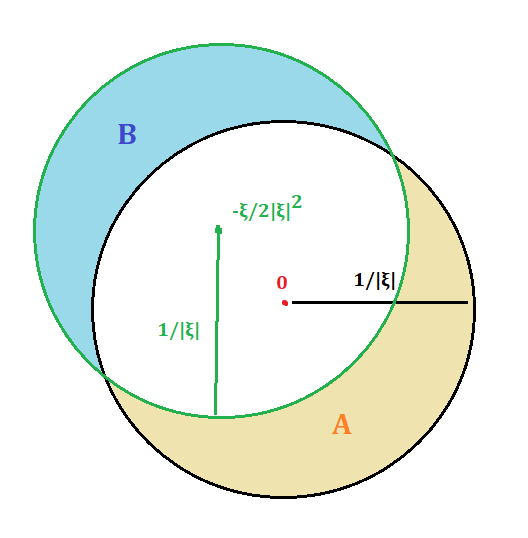
\includegraphics[scale =0.5]{regions}
			\caption{$A$ is the region of integration $|x - \xi/2|\xi|^2| \leq 1/|\xi| \leq |x|$ and $B$ is the region of integration $|x| \leq 1/|\xi| \leq |x - \xi/2|\xi|^2|$.}
		\end{center}	
		\end{figure}	
		
	The first integral \textsc{I} is controlled by the uniform Hormander condition for $K_\epsilon$, 
		\[ |\textsc{I}| \lesssim \int_{|x|> 1/|\xi|} |K_\epsilon (x) - K_\epsilon (x - \xi/2|\xi|^2)| \, dx \lesssim 1.  \]
	By the triangle inequality, $|x| \leq 1/|\xi| \leq |x - \xi/2|\xi|^2|$ implies $1/|\xi| \leq |x - \xi/2|\xi|^2| \leq 3/2|\xi|$. Thus the second integral \textsc{II} is controlled by the size condition, 
		\[ |\textsc{II}| \lesssim \int_{1/2|\xi| \leq |x - \xi/2|\xi|^2| \leq 3/2|\xi|} |K_\epsilon (x - \xi/2|\xi|^2)| \, dx \lesssim 1. \]
	Arguing analogously gives the result for \textsc{III}. We conclude $||\widehat{K_\epsilon}||_{L^\infty} \lesssim 1$ uniformly in $\epsilon$, as desired. 		
\end{proof}

\begin{theorem}
	Let $K \in L^1_{\loc} (\R^d \setminus 0)$ satisfy the cancellation, size, and smoothness conditions,
	\begin{align*}
		 \left| \int_{R_1 < |x| < R_2} K(x) \, dx \right| 
		 	&\lesssim 1 \qquad \text{uniformly in $0 < R_1 < R_2 < \infty$}, \\
		 \int_{R < |x| < 2R} |K(x)| \, dx 
		 	&\lesssim 1 \qquad \text{uniformly in $0 < R < \infty$}, \\
		 \int_{|x| > 2|y|} |K(x - y) - K(x)| \, dx 
		 	&\lesssim 1 \qquad \text{uniformly in $y \neq 0$,}
	\end{align*}
	and suppose further that the principal value distribution $\pv K$ exists, i.e.
		\[ \lim_{\epsilon \to 0} \int_{\epsilon < |x| < 1} K(x) \, dx. \]
	Then the convolution operator $T f := \pv K * f$ is a Calderon-Zygmund operator such that $K_\epsilon * f \to Tf$ pointwise a.e. for $f \in \cS (\R^d)$. \label{thm:czconvolution}
\end{theorem}

\begin{remark}
	The cancellation condition and existence of the principal value distribution are implied by the stronger cancellation condition 
		\[ \int_{R_1 < |x| < R_2} K(x) \, dx = 0 \qquad \text{for all $0 < R_1 < R_2 < \infty$}. \]
	As an example, the kernel of the Hilbert transform satisfies this strong cancellation condition. Another useful example with applications to partial differential equations are the Riesz transforms, which correspond to the kernels $K_j (x) := x_j/|x|^{d + 1}$.
\end{remark}

\subsection{Singular integrals}

A \emph{singular kernel} is a function $K : \R^d \times \R^d \to \C$ satisfying the Holder-type regularity estimates
	\begin{align*}
			|K(x, y) - K(x, z)| 
				&\lesssim \frac{|y - z|^\delta}{|x - y|^{d + \delta}},	\qquad \text{whenever } |x - y| > 2|y - z|,\\
			|K(x, y) - K(w, y)| 
				&\lesssim \frac{|x - w|^\delta}{|x - y|^{d + \delta}},	\qquad \text{whenever } |x - y| > 2|x - w|	,
		\end{align*}
for some Holder exponent $0 < \delta \leq 1$ and the decay estimate
	\[ |K(x, y)| \lesssim \frac{1}{|x - y|^d}. \]
Similar to the case of the Hilbert transform, singular kernels admit a logarithmic singularity along the diagonal $x = y$, so we cannot apply Schur's test to prove boundedness of the corresponding operator. As one might expect, showing a singular kernel gives rise to a Calderon-Zygmund operator is far more subtle than the translation-invariant case, and so we will reserve this story for another time and assume there exists a Calderon-Zygmund operator $T: L^2 (\R^d) \to L^2 (\R^d)$ with $K$ as its kernel. 

The decay estimate implies that the kernel is locally integrable in each variable on $\R^d \setminus 0$. We can therefore define the truncated operator
	\[ T_\epsilon f(y) := \int_{|x - y| > \epsilon} K(x, y) f(x) \, dx \]
for $f \in C^\infty_c (\R^d)$. We say that $T$ is a \emph{singular integral operator} if 
	\[ \lim_{\epsilon \to 0} T_\epsilon f(y) = Tf(y) \]
for a.e. $y \in \R^d$ and $f \in L^p (\R^d)$ for $1 < p < \infty$. To make sense of the problem, we need to establish conditions under which the limit on the left exists. Following an argument analogous to the proof of Lemma \ref{lem:pv}, we obtain
\begin{lemma}
	Let $K : \R^d \to \R^d \to \C$ be a singular kernel and $f \in C^\infty_c (\R^d)$. Then the limit
		\[ \lim_{\epsilon \to 0} T_\epsilon f(y)\]
	exists if and only if the limit 	
		\[ \lim_{\epsilon \to 0} \int_{\epsilon < |x - y| < 1} K(x, y) \, dx \]	
	exists.	
\end{lemma}

It is typical to have $T_\epsilon f \to Tf$ pointwise a.e. for $f \in C^\infty_c (\R^d)$, such as in the case of convolution kernels in Theorem \ref{thm:czconvolution}. This would reduce the problem to showing the set of functions for which $T_\epsilon f \to Tf$ pointwise a.e. forms a closed subspace of $L^p (\R^d)$, which in turn is implied by weak-type bounds for the corresponding \emph{maximal operator}
	\[ T^* f(y) := \sup_{\epsilon > 0} |T_\epsilon f(y)|.\]	

\begin{lemma}[Cotlar's inequality]
	Let $T : L^2 (\R^d) \to L^2 (\R^d)$ be a Calderon-Zygmund operator with singular kernel and let $0 < \nu \leq 1$. Then 
		\[ T^* f(y) \lesssim_\nu M(|Tf|^\nu) (y)^{1/\nu} + Mf(y) \]
	uniformly for $f \in C^\infty_c (\R^d)$ and a.e. $y \in \R^d$. 
\end{lemma}

\begin{proof}
	Fix $\epsilon > 0$, we aim to show 
		\[ T_\epsilon f(y) \lesssim_\nu M(|Tf|^\nu) (y)^{1/\nu} + Mf(y). \]
	Suppose that $|y - z| < \epsilon/2$, then applying the Holder-type estimates on the kernel, the second follows from a dyadic decomposition of the region $|x - y| > \epsilon$ we obtain
		\begin{align*}
			|T(f \mathbb 1_{|x - y| > \epsilon}) (z) - T(f \mathbb 1_{\mathbb 1_{|x - y| > \epsilon}}) (y)|
				&\leq \int_{|x - y| > \epsilon} |K(x, z) - K(x, y)| \, |f(x)| \, dx  \\
				&\lesssim |y - z|^\delta \int_{|x - y| > \epsilon} \frac{|f(x)|}{|x - y|^{d + \delta}} \, dx \\
				&\lesssim \epsilon^\delta \sum_{N \in 2^\N} \int_{N\epsilon < |x - y| < 2N \epsilon} \frac{|f(x)|}{|x - y|^{d + \delta}} \, dx \\
				&\lesssim  \sum_{N \in 2^\N} N^{-\delta} \frac{1}{(N\epsilon)^d}\int_{|x - y| < 2N \epsilon} |f(x)| \, dx \lesssim Mf(y).
		\end{align*}	
	Observe that $T (f \mathbb 1_{|x - y| > \epsilon}) (y) = T_\epsilon f(y)$. Hence by the triangle inequality and the inequality above we have
		\[ |T_\epsilon f(y)| \leq Mf (y)+ |T f(z)|+ |T(f \mathbb 1_{|x - y| < \epsilon}) (z)|.\]
	It remains to choose $z$ such that the last two terms are controlled by $M(|Tf|^\nu) (y)^{1/\nu}$ and $Mf(y)$ respectively. To control $|Tf(z)|$, we apply Chebyshev's inequality, 
		\[ |\{ z : |z - y|< \epsilon \text{ and } |Tf(z)| > \lambda \}| \leq \frac{1}{\lambda^\nu} \int_{|z - y| < \epsilon} |Tf(z)|^\nu \, d z \leq \frac{|B_{\epsilon} (y)|}{\lambda^\nu} M(|Tf|^\nu))(y).\]
	Choosing $\lambda > 4^{1/\nu} M(|Tf|^\nu) (y)^{1/\nu}$, we obtain
		\[ |\{ z : |z - y|< \epsilon \text{ and } |Tf(z)| > \lambda \}| \leq \frac14 |B_{\epsilon} (y)|. \]	
	To control $|T(f \mathbb 1_{|x - y| < \epsilon})(z)|$, it follows from the weak-type $(1 ,1)$ inequality for $T$ that
		\[ |\{ z : |z - y|< \epsilon \text{ and } |T(f \mathbb 1_{|x - y| < \epsilon})(z)| > \lambda \}| \leq \frac{C}{\lambda} \int_{|x - y| < \epsilon} |f(x)| \, dx \leq \frac{C \, |B_\epsilon (y)|}{\lambda} Mf (y). \]	
	Choosing $\lambda > 4C Mf (y)$, we obtain
		\[  |\{ z : |z - y|< \epsilon \text{ and } |T(f \mathbb 1_{|x - y| < \epsilon})(z)| > \lambda \}| \leq \frac14 |B_\epsilon (y)|. \]
	Thus there exists $z \in B_{\epsilon} (y)$, i.e. $|z - y| < \epsilon$, such that $|Tf(z)| < \lambda$ and $|T(f\mathbb 1_{|x - y| < \epsilon})| < \lambda$. Choosing $\lambda$ optimally completes the proof. 
\end{proof}

\begin{theorem}
	Let $T: L^2 (\R^d) \to L^2 (\R^d)$ be a Calderon-Zygmund operator with singular kernel, then its maximal operator $T^*$ is weak-type $(1, 1)$ and strong-type $(p, p)$ for $1 < p < \infty$. 
\end{theorem}

\begin{proof}
	The strong-type $(p, p)$ inequality follows immediately from Cotlar's inequality for $\nu = 1$ since the Hardy-Littlewood maximal function and $T$ are strong-type $(p, p)$. 	For the weak-type $(1, 1)$ inequality, fix $\nu < 1$, then it suffices by Cotlar's inequality and the Hardy-Littlewood weak-type $(1, 1)$ inequality to show
		\[  ||M(|Tf|^\nu)^{1/\nu} ||_{L^{1, \infty}} \lesssim ||f||_{L^1}. \]
	By Hunt's interpolation theorem, the Hardy-Littlewood maximal operator	is bounded on $L^{1/\nu, \infty} (\R^d)$. Combined with the weak-type $(1, 1)$ inequality for $T$, we obtain
		\[ ||M(|Tf|^\nu)^{1/\nu} ||_{L^{1, \infty}} \sim ||M (|Tf|^\nu)||_{L^{1/\nu, \infty}}^{1/\nu} \lesssim |||Tf|^\nu||_{L^{1/\nu, \infty}}^{1/\nu} \sim ||Tf||_{L^1, \infty} \lesssim ||f||_{L^1} \]
	as desired. 
\end{proof}

\begin{theorem}
	Let $T: L^2 (\R^d) \to L^2 (\R^d)$ be a Calderon-Zygmund operator with singular kernel such that 
		\[ \lim_{\epsilon \to 0} T_\epsilon f = Tf \]
	pointwise a.e. for all $f \in C^\infty_c (\R^d)$. Then the convergence above continues to hold for $f \in L^p (\R^d)$ both pointwise and in norm for $1 < p < \infty$. 
\end{theorem}

\begin{proof}
	Pointwise convergence follows from boundedness of the maximal operator. Convergence in norm follows from dominated convergence theorem and $T^* f \in L^p (\R^d)$. 
\end{proof}

\begin{remark}
	We cannot use the same argument to establish convergence in norm for $p = 1$. Nevertheless, this result still holds provided that $Tf \in L^1 (\R^d)$; this is due to Calderon and Capri. 
\end{remark}

\subsection{Fourier multipliers}

If $m :\R^d \to \C$ is a tempered distribution, we can define the \emph{Fourier multiplier} $m(D) : \cS (\R^d) \to \cS (\R^d)^*$ implicitly in frequency space by
	\[ \widehat{m(D) f} (\xi) := m(\xi) \widehat f(\xi), \]
or explicitly in physical space by
	\[ m(D) f(x) := (\widecheck m * f) (x). \]
The function $m$ is known as the \emph{symbol} of the operator $m(D)$. We formally have the multiplier calculus
	\begin{align*}
		m(D)^*
			&= \overline m(D), \\
		m_1 (D) + m_2 (D)
			&= (m_1 + m_2)(D), \\
		m_1 (D) m_2 (D)
			&= (m_1 m_2) (D).		
	\end{align*}
In particular, Fourier multipliers commute with each other. Just as in Section \ref{sec:convop} we determined conditions on the convolution kernel under which the corresponding operator formed a Calderon-Zygmund operator, we want to find conditions on $m$ under which the operator $m(D)$ forms a Calderon-Zygmund operator. 

\begin{theorem}[Hormander-Mikhlin multiplier theorem]
	Let $m \in C^{d + 2}_{\loc} (\R^d \setminus 0)$ obey the homogeneous symbol estimate of order zero
		\[ |D^\alpha_\xi m(\xi)| \lesssim |\xi|^{-|\alpha|} \]
	uniformly in $\xi \neq 0$ for all $0 \leq |\alpha| \leq d + 2$. Then $m(D)$ is a Calderon-Zygmund operator. 	
\end{theorem}
\begin{proof}
	The boundedness condition $m \in L^\infty (\R^d)$ is clearly satisfied. \textit{A priori}, we only know that the kernel $\widecheck m$ is a tempered distribution. We claim that it is in fact a singular kernel satisfying the gradient estimate, which would complete the proof. To this end, we localise in frequency space, choosing a non-negative bump function $\phi \in C^\infty_c (\R^d)$ supported on the unit ball, and defining
		\[ \psi_N (\xi) := \phi(\xi/2N) - \phi(\xi/N) \] 
	for $N \in 2^\Z$. By construction, $\psi_N$ are localised at dyadic frequencies $|\xi| \sim N$ and form a partition of unity $\sum_N \psi_N \equiv 1$. We can write
		\[ m = \sum_{N \in 2^\Z} m \psi_N =: \sum_{N \in 2^\Z} m_N  \]
	with convergence pointwise and in the sense of tempered distributions. It follows from the Paley-Wiener theorem that the kernels $\widecheck{m_N}$ are smooth. Furthermore, they satisfy by the Fourier transform strong-type $(1, \infty)$ inequality
		\begin{align*}
			||x^\alpha \widecheck{m_N} ||_{L^\infty_x} 
			 	&\lesssim ||\partial^\alpha_\xi  m_N||_{L^1_\xi} ,\\
			 ||x^\alpha \nabla \widecheck{m_N} ||_{L^\infty_x} 
			 	&\lesssim ||\partial^\alpha_\xi (\xi m_N)||_{L^1_\xi} .
		\end{align*} 
	Using the product rule and the control on the derivatives of $m$, the right-hand sides are controlled pointwise by 
		\begin{align*}
			\left|\partial^\alpha_\xi m_N\right| 
				&\lesssim \sum_{\beta + \gamma = \alpha} | \partial^{\beta}_\xi  m| \, |\partial^\gamma_\xi \psi_N| \lesssim_\alpha \sum_{\beta + \gamma = \alpha} |\xi|^{- |\beta|} N^{-|\gamma|} |\partial_\xi^\gamma \psi (\xi/N)|, \\
			\left|\partial^\alpha_\xi (\xi m_N)\right| 
				&\lesssim \sum_{\beta + \gamma = \alpha} | \partial^{\beta}_\xi (\xi m)| \, |\partial^\gamma_\xi \psi_N| \lesssim_\alpha \sum_{\beta + \gamma = \alpha} |\xi|^{1 - |\beta|} N^{-|\gamma|} |\partial_\xi^\gamma \psi (\xi/N)|.   
		\end{align*}	
	Therefore
		\begin{align*}
			||\partial^\alpha_\xi m_N||_{L^1_\xi}
				&\lesssim \sum_{\beta + \gamma = \alpha} \int_{|\xi| \sim N} |\xi|^{ - |\beta|} N^{-|\gamma|} d \xi \lesssim \sum_{\beta + \gamma = \alpha} N^{ d - |\beta| - |\gamma|} \sim N^{d - |\alpha|}, \\
			||\partial^\alpha_\xi (\xi m_N)||_{L^1_\xi}
				&\lesssim \sum_{\beta + \gamma = \alpha} \int_{|\xi| \sim N} |\xi|^{1 - |\beta|} N^{-|\gamma|} d \xi \lesssim \sum_{\beta + \gamma = \alpha} N^{1 + d - |\beta| - |\gamma|} \sim N^{1 + d - |\alpha|}. 
		\end{align*}
	Collecting the inequalities above and taking $|\alpha| = 0$ and $|\alpha| = d + 2$, we obtain
		\begin{align*}
			|\widecheck{m_N} (x)|
				&\lesssim \min\{ N^d, |x|^{-d - 2} \}\\
			|\nabla \widecheck{m_N} (x) | 
				&\lesssim \min \{ N^{d + 1}, N^{-2} |x|^{- d - 2} \}.
		\end{align*}	 
	These inequalities imply that the convergence $\widecheck m = \sum_N \widecheck{m_N}$ holds in $C^1_{\loc} (\R^d \setminus 0)$ and furthermore
		\begin{align*} 
			|\widecheck m (x)|
				&\lesssim \sum_{N \in 2^\Z} |\widecheck{m_N} (x)| \lesssim \sum_{N \leq |x|^{-1}} N^{d} + \sum_{N > |x|^{-1}} N^{-2}|x|^{-d - 2} \lesssim |x|^{-d},\\
			|\nabla \widecheck m (x)|
				&\lesssim \sum_{N \in 2^\Z} |\nabla \widecheck{m_N} (x)| \lesssim \sum_{N \leq |x|^{-1}} N^{d + 1} + \sum_{N > |x|^{-1}} N^{-1} |x|^{-d - 2} \lesssim |x|^{-d - 1}. 
		\end{align*}	
	This proves the claim and thereby the theorem. 	
\end{proof}

\begin{remark}
	As an application to partial differential equations, define the \emph{Riesz transforms} $R_j := i D_j/|D|$ as multipliers with symbols $m_j := i\xi_j/|\xi|$. It is easy to verify that $m_j$ obey the homogeneous symbol estimates, so, writing $\partial_j \partial_j = - R_j R_k \Delta$, we obtain the \textit{elliptic regularity estimate}
		\[ ||\partial_j \partial_k f||_{L^p} \lesssim_{d, p} ||\Delta f||_{L^p} \]
	for all $f \in \cS (\R^d)$ and $1 < p < \infty$. 	
\end{remark}

\section{Vector-valued operators}

We can generalise much of the preceding discussion concerning scalar-valued functions to functions taking values in Banach spaces. Let $X$ and $Y$ be Banach spaces and denote by $B(X, Y)$ the bounded linear maps from $X$ to $Y$ endowed with the usual operator norm. For $f : \R^d \to X$, a \textit{vector-valued integral operator} takes the form
	\[ Tf(y) := \int_{\R^d} K(x, y) f(x) \, dx \]
where $K : \R^d \times \R^d \to B(X, Y)$ is the \textit{kernel}. 

\iffalse
\subsection{Christ-Kiselev lemma}
\begin{theorem}[Christ-Kiselev lemma]
	For $1 \leq p < q \leq \infty$, let $T: L^p (\R ; X) \to L^q (\R ; Y)$ be a bounded vector-valued integral operator with kernel $K : \R \times \R \to B(X, Y)$. Then $S : L^p (\R; X) \to L^q (\R; Y)$ given by 
		\[ S g(t) := \int_{-\infty}^t K(t, s) g(s) \, ds \]
	is also a bounded vector-valued integral operator. 	
\end{theorem}

The Christ-Kiselev lemma is the key tool for proving the inhomogeneous Strichartz estimates. Consider the initial data problem for the inhomogeneous linear Schrodinger equation 
	\begin{align*}
		i \partial_t + \Delta u
			&= F, \\
		u_{|t = 0}
			&= u_0.	
	\end{align*}
By Duhamel's principle, the solution takes the form
	\[ u(t) = e^{i t \Delta} u_0 + i \int_0^t e^{i (t - s) \Delta} F(s) \, ds. \]
The homogeneous Strichartz estimate states that 
	\[ ||e^{i t \Delta} u_0||_{L^{q}_t L^r_x} \lesssim ||u_0||_{L^2_x}  \]
for $2 \leq q, r \leq \infty$ satisfying $(q, r, d) \neq (2, \infty, 2)$ and 
	\[ \frac{2}{q} + \frac{d}{r} = \frac{d}{2}. \]			
\fi

\subsection{Vector-valued Calderon-Zygmund operators}

A \emph{vector-valued Calderon-Zygmund kernel} is a function $K : \R^d \times \R^d \to B(X, Y)$ satisfying the \emph{Hormander condition}:
	\begin{align*}
		\int_{|x - y| > 2|y - z|} ||K(x, y) - K(x, z)||_{B(X, Y)} \, dx &\lesssim 1 \qquad \text{uniformly for a.e. $y \neq z$}, \\
		\int_{|x - y| > 2|x - w|} ||K(x, y) - K(w, y)||_{B(X, Y)} \, dy &\lesssim 1 \qquad \text{uniformly for a.e. $x \neq w$}.
	\end{align*}
We say that a bounded linear operator $T: L^2 (\R^d; X) \to L^2 (\R^d;Y)$ is a \emph{vector-valued Calderon-Zygmund operator} if there exists a vector-valued Calderon-Zygmund kernel $K$ for which 
	\begin{equation*}
		Tf(y) = \int_{\R^d} K(x, y) f(x) \, dx
	\end{equation*}
whenever $f \in L^2 (\R^d; X)$ is compactly supported and $y$ lies outside the support of $f$. The Calderon-Zygmund decomposition and real interpolation continues to hold in the vector-valued setting, as the proofs depended only on the norm of the function. The only tool which does not freely carry over is duality $L^p (\R^d; Y)^* = L^{p'} (\R^d ; Y^*)$, and so a little more work is needed to establish the strong-type $(p, p)$ inequality for $2 < p < \infty$. We leave this as an exercise for the reader. 

\begin{theorem}
	If $T: L^2 (\R^d; X) \to L^2 (\R^d; Y)$ is a vector-valued Calderon-Zygmund operator, then it satisfies the weak-type $(1, 1)$ and strong-type $(p, p)$ inequalities for $1 < p < \infty$. 
\end{theorem}

As an application, we can establish the \textit{Littlewood-Paley inequality}. Let $\phi  \in C^\infty_c (\R^d)$ satisfy $0 \leq \phi \leq 1$ and 
\begin{align*}
	\phi(x) 
		:= 
		\begin{cases}
			1 , 				&|x| \leq 1.4, \\
			0, 				&|x| > 1.42. 
		\end{cases}
\end{align*}
Define
	\[ \psi_N (\xi) := \phi(\xi/N) - \phi(2\xi/N)  \]
for $N \in 2^\Z$. By construction, $\psi_N$ are localised at dyadic frequencies $|\xi| \sim N$ and form a partition of unity $\sum_N \psi_N \equiv 1$. Given $f \in \cS (\R^d)^*$, we define its \emph{Littlewood-Paley projection} to frequency $|\xi| \sim N$ by
	\begin{align*}
		P_N f := \psi_N (D) f. 
	\end{align*}	
The name ``projection'' is a bit of a misnomer; the multipliers $P_N$ fail to be true projections in the sense that by choosing smooth cutoffs in frequency space rather than sharp cutoffs, we have $P_N P_N \neq P_N$. Nevertheless, a slightly modified statement holds; define the \emph{fattened Littlewood-Paley projections} to frequencies $|\xi| \sim N$ and their corresponding symbols by
	\[ \widetilde{P_N} := P_{\frac{N}{2}} + P_{N} + P_{2N},\qquad  \widetilde{\psi_N} := \psi_{\frac{N}{2}} + \psi_N + \psi_{2N}. \]
Since $\widetilde{\psi_N} \equiv 1$ on the support of $\psi_N$, it follows that $\widetilde{P_N} P_N = P_N$.

\begin{theorem}[Littlewood-Paley inequality]
	Let $1 < p < \infty$ and $f \in L^p (\R^d)$, define the \emph{Littlewood-Paley square function} by 
	\[ Sf := \left( \sum_{N \in 2^\Z} |P_N f|^2 \right)^{1/2}. \]
	Then 
		\[ ||S f||_{L^p} \sim ||f||_{L^p}. \]
\end{theorem}

\begin{proof}
	The inequality $||Sf||_{L^p} \lesssim ||f||_{L^p}$ is equivalent to establishing that the operator $T: L^2 (\R^d) \to L^2 (\R^d ; \ell^2)$ defined by 
		\[ Tf := ( P_N f )_{N \in 2^\Z}  \]
	is a Calderon-Zygmund operator. The corresponding kernel $K: \R^d \to B(\C, \ell^2)$ is
		\[ K(x) = (\widecheck{\psi_N} (x))_{N \in 2^\Z}. \]
	Since $\sum_N \psi_N \equiv 1$, it follows from Plancharel's theorem that $T$ is strong-type $(2, 2)$. The symbols $\psi_N$ obey the estimates from the Hormander-Mikhlin multiplier theorem, so following the proof we conclude $K$ satisfies the Hormander condition and therefore $T$ is a Calderon-Zygmund operator. 
	
	For the reverse inequality, we argue by duality, remarking that $\widetilde P_N$ is self-adjoint and the argument above continues to hold replacing the square function $Sf$ with the fattened square function $\widetilde S f$. The convergence $f = \sum_N P_N f = \sum_N \widetilde{P_N} P_N f$ holds in $L^p (\R^d)$, so by duality, Cauchy-Schwartz in $N$, and Holder's inequality in $x$, 
		\begin{align*}
			||f||_{L^p}
				&=\sup_{||g||_{L^{p'}  } \leq 1} \sum_N\langle  \widetilde P_N P_N f, g \rangle = \sup_{||g||_{L^{p'}  } \leq 1} \sum_N \langle P_N f, \widetilde P_N  g \rangle \leq \sup_{||g||_{L^{p'}  } \leq 1} ||S f||_{L^p} ||\widetilde S g||_{L^{p'}} \lesssim ||Sf||_{L^p}.
		\end{align*}
	This completes the proof. 	
\end{proof}

\bibliographystyle{alpha}
\bibliography{biblio}

\end{document}